\chapter{Model checking for Markov decision processes}

Storm allows to model-check discrete-time and continuous-time models, i.e.,
verify that properties hold in states of models. This
chapter will cover discrete-time model checking via a \textit{probabilistic branching-time logic}. We will detail the syntax, the semantic and model checking algorithms of this logic.
We will see that it is possible to extend this logic to support weights of MCs and MDPs. Then, we will see that it is
possible to formulate requests with this logic to solve
problems we encountered in the first chapter and that we
will address in the following chapter, covering multi-objective support for MDPs. \\

As model checking for MDPs uses the notion of strategy to resolve nondeterminism,
we first need to introduce the probabilistic branching time logic for MCs.

\section{Probabilistic computational tree logic}
\textit{Probabilistic computational tree logic} (or \textbf{PCTL}, for short) is a \textit{branching-time temporal logic}.
This logic allows to verify probabilistic systems via an
%probabilistic
execution tree, actually named \textit{computational tree}. For a given system, this tree consists of an infinite unfolding of this system, considering
all branching possibilities.
%Thus, it is actually an MC with an infinite tree as underlying graph.
The key idea of this tree is that each branch of a node leads to a possible future of this node.
So, this tree is highly linked to cylinder sets.  Possible futures of a node actually correspond to paths of the cylinder set for which the prefix leads the root to the node in the tree.
\begin{example}[\textit{Computational tree of an MC}]
Let $\mathcal{M}$ be the MC of the figure \ref{ct1}. The computational tree of $\mathcal{M}$ starting from the state $s_0$ is
given in the figure \ref{ct2}. We clearly see in this tree that each possible future of a node $s^*$ actually corresponds to a state $s'_n$ of a path $\pi = s'_0 \dots s'_k \dots s'_n \dots \in Cyl(s'_0 \dots s'_k)$ such that $s'_0 = s_0$, $s'_k=s^*$ and $k < n$.
For example, $s_1$ is a possible future of the node $s_0$ (for which the prefix is $s_0s_0$) because the path $\pi = s_0s_0s_0(s_1s_2)^\omega$ is in $Cyl(s_0s_0)$.
\begin{figure}[h]
  \begin{minipage}{0.4\linewidth}
    \centering
    \includegraphics[width=0.8\linewidth]{resources/CLT_unfolding_1}
    \captionsetup{justification=centering}
    \captionof{figure}{MC $\mathcal{M}$ with $3$ states, $s_0, s_1$ and $s_2$, and $2$ atomic propositions, $a$ and $b$}\label{ct1}
  \end{minipage}
  \begin{minipage}{0.6\linewidth}
    \centering
    \includegraphics[width=0.8\linewidth]{resources/CLT_unfolding_2}
    \captionsetup{justification=centering}
    \captionof{figure}{Computational tree of $\mathcal{M}$ starting from $s_0$}\label{ct2}
  \end{minipage}
\end{figure}
We will see that it is possible to express formulae in PCTL describing states properties of the system like the following one:
\begin{center}
``\textit{Do all executions starting from the state $s_0$ always eventually reach $b$ with a nonzero probability ?}''
\end{center}
Model checking algorithms of PCTL will answer \textit{yes} to this.
Intuitively, if we refer to the computational tree,
%we see that it is possible to reach a node labeled with $b$,
%from any node of the tree,
%via a path from this node that has a nonzero probability.
%we see that it is possible to reach a node labelled with $b$ from any node of the tree and, each cylinder set
%for which the prefix leads the root to any node has a nonzero probability:
we see that a node labelled with $b$ appears in the future of any node $s^*$ of the tree. Furthermore, there exists an index $n$ for each path $\pi = s'_0 s'_1 s'_2 \dots s'_n \dots \in Cyl(s'_0 \dots s'_k)$, where $s'_0 \dots s'_k$ is the prefix that leads the root to the node $s^* = s'_k$ in the tree, such that $k <n$ and $s'_n$ is labelled with $b$, except for the path $s_0^\omega$ (corresponding to the left path in the computational tree).
Since this path has a zero probability, we have that this property is verified with a probability one from the state $s_0$.
We will see in this chapter how to verify formally each property of this type.
%let $\hat{\pi} = s'_0 \dots s'_n$ be a finite path of $\mathcal{M}$, starting from the state $s_0$ of $\mathcal{M}$ and referring to a finite path starting from the root of the tree. If there exists an index $k$, such that $1 \leq k \leq n$ and $s'_k = s_1$, then $\mathbb{P}_{s_0}(Cyl(s'_0 \dots s'_k \dots s'_n)) = \prod_{i=0}^{k-1} \Delta(s'_i, s'_{i+1}) \cdot 1^\omega = \frac{1}{10}^{k-1}$.
%Else, $\hat{\pi} = s_0^{n+1}$ and $\mathbb{P}_{s_0}(Cyl(s_0^{n+1})) = \frac{1}{10}^n$.
%Furthermore, all executions starting from $s_0$ has a probability one to always eventually reach a state labeled with $b$: the only path starting from $s_0$ that does not allow it is the path $s_0^\omega$ (corresponding to the left path in the computational tree) and has a zero probability.
\end{example}

\subsection{Syntax and semantic}
PCTL has a two stages syntax where PCTL formulae are classified into state and path formulae. Intuitively, \textit{state formulae} are assertions about atomic propositions in a state $s$ and about probabilities over their branching structure, i.e., probabilities of \textit{path formulae} starting from $s$. Actually, a path formula will impose conditions on a set of paths and this path formula will be quantified
by probability bounds.

\begin{definition}[\textbf{Syntax of PCTL}]
Let $AP$ be a set of atomic propositions,
\begin{itemize}
  \item PCTL \textit{state formulae} are formed according the following grammar:
  \[
    \Phi ::= true \;\; | \;\; a \;\; | \;\; \Phi_1 \wedge \Phi_2 \;\; | \;\; \neg \Phi \;\; | \;\; \mathcal{P}_J(\phi)
  \]
  where $a \in AP$ is an atomic proposition, $J \subseteq [0, 1]$ gives probability bounds and $\phi$ is a path formula.
  \item PCTL \textit{path formulae} are formed according the following grammar:
  \[
  \phi ::= \bigcirc \Phi \;\; | \;\; \Phi_1 \U \Phi_2 \;\; | \;\; \Phi_1 \U^{\leq n} \Phi_2
  \]
  where $\Phi$, $\Phi_1$ and $\Phi_2$ are state formulae and $n \in \mathbb{N}$.
\end{itemize}
\end{definition}
Intuitively, $\mathcal{P}_J(\phi)$ specify that the probability of paths satisfying the path formula $\phi$ must be in the interval $J$. A path formula is formed by temporal operators, like $\bigcirc$ and $\U$, with $\U^{\leq n}$ being $\U$ bounded by a maximum number of steps.  There exists some other linear temporal operators, dealing with paths of the system (cf. figure \ref{ltl}). These operators can be derived from the PCTL grammar:
let $J \in [0, 1]$ giving probability bounds, $\Phi$ be a state formula and $n \in \mathbb{N}$ be a number of steps,

\makeatletter
\newcommand*\bigcdot{\mathpalette\bigcdot@{.5}}
\newcommand*\bigcdot@[2]{\mathbin{\vcenter{\hbox{\scalebox{#2}{$\m@th#1\bullet$}}}}}

\makeatother
\begin{flalign}
  &\bigcdot \; \mathcal{P}_J(\Diamond \Phi) \equiv \mathcal{P}_J(true \U \Phi) \tag{\textit{eventually} probability} \\
  &\bigcdot \; \mathcal{P}_J(\Diamond^{\leq n} \Phi) \equiv \mathcal{P}_J(true \U^{\leq n} \Phi) \tag{\textit{bounded enventually} probability} \\
  &\bigcdot \; \mathcal{P}_J(\Box \Phi) \equiv
    \neg \mathcal{P}_J(\Diamond \neg \Phi)
    \tag{\textit{always} probability}
\end{flalign}

\begin{figure}[h]
  \centering
  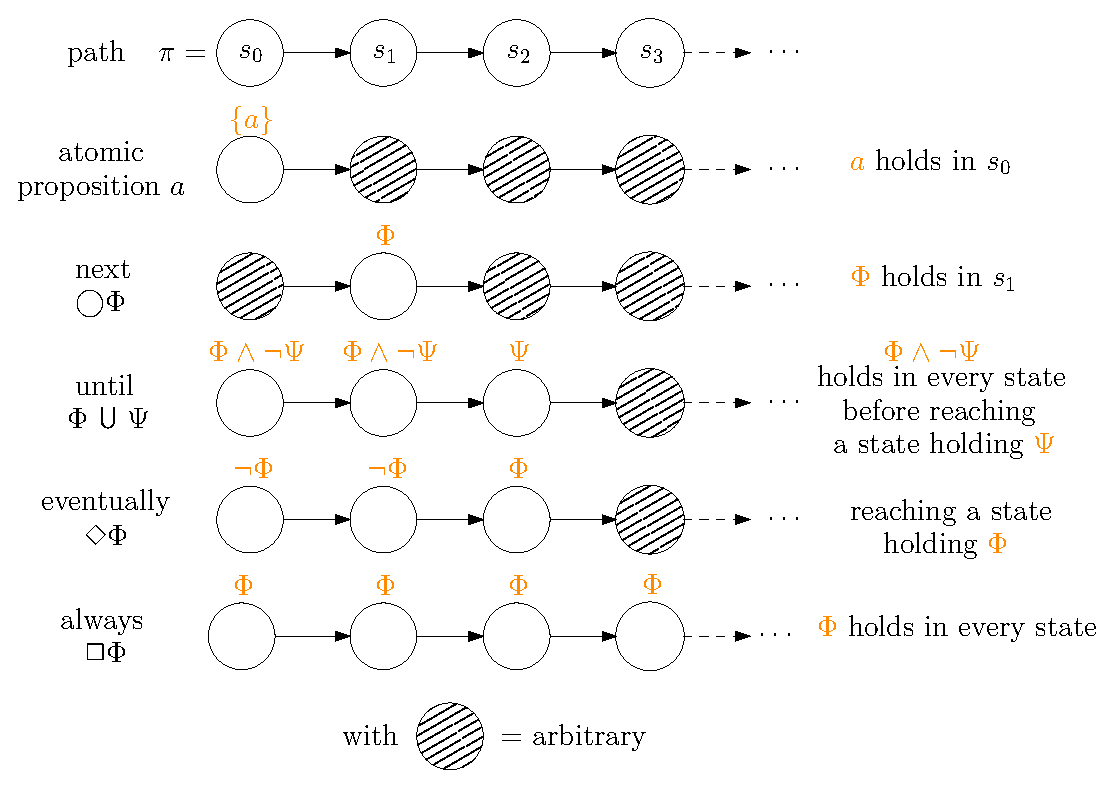
\includegraphics[width=0.85\linewidth]{resources/LTL}
  \caption{Intuitive semantic of linear temporal operators}\label{ltl}
\end{figure}

\begin{definition}[\textbf{Semantic of PCTL}]
  Let $\mathcal{M} = (S, A, \Delta, AP, L)$ be an MC and $s \in S$, be a state of $\mathcal{M}$,
  \begin{flalign*}
  \intertext{$s \models \Phi$ iff the state formula $\Phi$ holds in the state $s$, i.e.,}
    &\bigcdot\; s \models true, &&&\\
    &\bigcdot\; s \models a &\text{ iff }& a \text{ is a label of $s$, i.e., } a \in L(s),&\\
    &\bigcdot\; s \models \Phi_1 \wedge \Phi_2&\text{ iff }& s \models \Phi_1 \text{ and } s \models \Phi_2,&\\
    &\bigcdot\; s \models \neg \Phi &\text{ iff }& s \not\models \Phi, &\\
    &\bigcdot\; s \models \mathcal{P}_J(\phi) &\text{ iff }& \mathbb{P}_s(\{ \pi \in Paths(s) \; | \; \pi \models \phi \}) \in J.& \\
  \intertext{Following a path $\pi = s_0s_1s_2\dots \in Paths(s)$, $\pi \models \phi$ iff $\pi$ satisfies the path formula $\phi$, i.e., }
  &\bigcdot\;\pi \models \Phi&\text{ iff }&s_0 \models \Phi,&\\
  &\bigcdot\;\pi \models \bigcirc\, \Phi&\text{ iff }&s_1 \models \Phi,&\\
  &\bigcdot\;\pi \models \Phi_1 \U \Phi_2 &\text{ iff }& \exists j \in \mathbb{N},\, s_j \models \Phi_2
    \text{ and } \forall i \in \mathbb{N}, \, i < j, \, s_i \models \Phi_1,&\\
  &\bigcdot\;\pi \models \Phi_1 \U^{\leq n} \Phi_2 &\text{ iff }& \exists j \in \mathbb{N}, \, j \leq n ,\, s_j \models \Phi_2
    \text{ and } \forall i \in \mathbb{N}, \,i < j, \, s_i \models \Phi_1.&\\
  \intertext{Additionally,}
  &\bigcdot\; \pi \models \Diamond \Phi&\text{ iff }& \exists j \in \mathbb{N}, \, s_j \models \Phi,&\\
  &\bigcdot\; \pi \models \Box \Phi&\text{ iff }& \forall j \in \mathbb{N}, \, s_j \models \Phi.&
  \end{flalign*}
\end{definition}
\begin{remark}[\textit{Measurability of path formulae}]
Since $\mathcal{P}_J(\phi)$ refers to probabilities, $\neg \mathcal{P}_J(\phi) = \mathcal{P}_{J'}(\phi)$ for any path formula $\phi$, with $J'=[0, 1] \setminus J$. Then, the event $\{ \pi \in Paths(s) \; | \; \pi \models \phi\}$ must be measurable to verify that $\mathcal{P}_J(\phi)$ holds in any state. We will see that these events can be formed through countable unions of cylinder sets, ensuring their measurability.
\end{remark}
\begin{remark}[\textit{Probabilistic satisfiability of path formulae}]
Let $\mathcal{M}$ be the MC of the figure \ref{pctlctl}.
\begin{figure}[h]
  \centering
  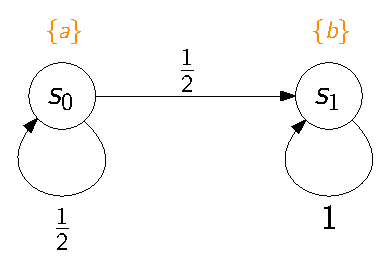
\includegraphics[width=0.25\linewidth]{resources/PCTL_CTL}
  \captionsetup{justification=centering}
  \caption{MC $\mathcal{M}$ with $2$ states, $s_0$ and $s_1$, and $2$ atomic propositions, $a$ and $b$}\label{pctlctl}
\end{figure}
\begin{itemize}
% \item Let assume that there exists a path $\pi \in Paths(s_0)$ starting from $s_0$ in $\mathcal{M}$ such that $\pi \not \models \phi$, for any PCTL path formula $\phi$. That does not mean that $s_0 \models \mathcal{P}_{<1}(\phi)$: take $\pi=s_0^\omega$ and $\phi = \Diamond b$, we have that $s_0^\omega \not \models \Diamond b$ and $\mathbb{P}_s(\Diamond \{s_1\}) = 1$.
% Then $s_0 \models \mathcal{P}_{=1}(\Diamond b)$.
  \item Let assume there exists a state $s$ in an MC such that $s \models \mathcal{P}_{=1}(\phi)$, for any path formula $\phi$. That does not mean that all paths $\pi \in Paths(s)$ satisfy $\phi$.
  Indeed, consider the MC $\mathcal{M}$ and take the state $s_0$ of $\mathcal{M}$, the path $s_0^\omega \in Paths(s_0)$ and the path formula $\Diamond b$. We have that $s_0 \models \mathcal{P}_{=1}(\Diamond b)$, because $\mathbb{P}_{s_0}(\Diamond \{s_1\})=1$, but we have that $s_0^\omega \not \models (\Diamond b)$.

  \item Let assume there exists a state $s$ in an MC such that there exists a path $\pi \in Paths(s)$, starting from this state $s$, such that $\pi \models \phi$, for any path formula $\phi$.
  That does not mean that $s \models \mathcal{P}_{> 0}(\phi)$.
  Indeed, consider the MC $\mathcal{M}$ and take the state $s_0$, the path $s_0^\omega \in Paths(s_0)$ and the path formula $\Box a$. We have that the path $s_0^\omega$ is the only path of $\mathcal{M}$ that verifies $\Box a$ (and thus, $s_0^\omega \models \Box a$).
  However, we have that $\mathbb{P}_s(\{s_0^\omega\})=0$. Then, $s_0 \models \mathcal{P}_{=0} (\Box a)$.
\end{itemize}
\end{remark}

\begin{definition}[\textbf{Satisfiability set for PCTL}]
  Let $\mathcal{M}=(S, \Delta, w, AP, L)$ be an MC and $\Phi$ be a PCTL state formula on $AP$. The \textit{satisfiability set} for the MC $\mathcal{M}$ is defined as follows:
  \[
    Sat(\Phi) = \{ s \in S \, | \, s \models \Phi \}
  \]
\end{definition}
